\documentclass[12pt]{article}
\usepackage[a4paper]{geometry}
\usepackage[utf8]{inputenc}
\usepackage{fancyhdr}
\usepackage{lastpage}
\usepackage{graphicx, wrapfig, subcaption, setspace, booktabs}
\usepackage{graphicx}
\usepackage[T1]{fontenc}
\usepackage[font=small, labelfont=bf]{caption}
\usepackage[protrusion=true, expansion=true]{microtype}
\usepackage[english]{babel}
\usepackage{sectsty}
\usepackage{url, lipsum}
\usepackage[T1]{fontenc}
\usepackage{icomma}
\usepackage{siunitx}
\usepackage{ragged2e}
\usepackage{amsmath}
\usepackage{comment}
\usepackage{enumerate}
\usepackage{anysize}
\newcommand{\HRule}[1]{\rule{\linewidth}{#1}}
\onehalfspacing
\setcounter{tocdepth}{5}
\setcounter{secnumdepth}{5}


%-------------------------------------------------------------------


\begin{comment}

\end{comment}
\begin{document}

\begin{titlepage}

\title{ \normalsize 
        \begin{center}
        
\includegraphics[height=6cm]{Logo.jpg}
        \end{center}
        \LARGE \textsc{\textbf{Universidad De Sonora}} \\ \bigskip
		\Large División de Ciencias Exactas y Naturales \\
        Licenciatura En Física \\ \bigskip
        \bigskip
        Física Computacional I
		\\ [0.1cm]  
		\HRule{2pt} \\
		\Large \textbf{{Evaluación 2}} \\
        \textit{\textbf{ Oscilador armónico amortiguado forzado con una fuerza de tipo sinoidal}}
		\HRule{2pt} \\
		\normalsize \vspace*{0.001\baselineskip}}
        
\date{\bigskip \Large Hermosillo, Sonora  \hspace*{\fill}  05 de abril de 2021}

        
\author{
		\Large\textbf{Ismael Espinoza Arias} \\ \bigskip
        \\ \bigskip
       \Large Profresor Carlos Lizárraga Celaya}
       \end{titlepage}
       \maketitle
       
\newpage
\pagestyle{plain}

%-------------------------------------------------------------------

\section{Introducción}


El siguiente reporte forma parte de la primera evaluación del semestre, de la materia de Física Computacional 1, por lo que, a lo largo de él, hablaremos sobre el procedimiento usado para llegar a lograr la práctica propuesta y sobre los resultados que obtuvimos en el transcurso de la actividad.\\

Para la realización de esta evaluación, fue necesario el uso de los temas antes vistos, como lo son los temas de álgebra lienal. Esta evaluación fue realizada con el propósito de lograr demostrar las habilidades aprendidas en el transcurso del curso de Física Computacional 1, donde aplicaremos los conocimientos que tenemos hasta el momento gracias a las 9 actividades ya realizadas anteriormente. A lo largo de este reporte veremos e interpretaremos los datos obtenidos de esta actividad de evaluación. 


%-------------------------------------------------------------------


\section{Antecedentes}


Antes de iniciar la actividad, entraremos un poco en contexto acerca del tema, como mencionamos anteriormente nos interesa resolver los 3 problemas que encontramos en la actividad, donde los resolveremos usando las herramientas ya antes adquiridas en cursos posteriores de álgrebra lineal y el mimso de física computacional. \\



%-------------------------------------------------------------------


\section{Problema 1}

El en el caso #1, nos encontramos resolviendo numericamente el ejercicio, donde establecimos nuestros datos, sustituimos los valores, ingresamos algunas condiciones iniciales y llegamos a calcular las soluciones deseadas con su respectiva gráfica.\\

\begin{center}
 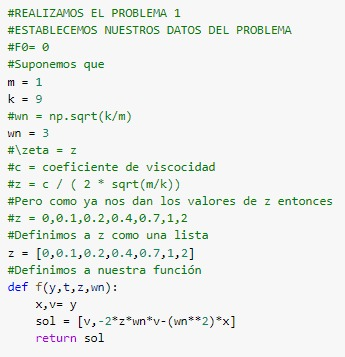
\includegraphics[height=15cm]{A1.jpeg}  
 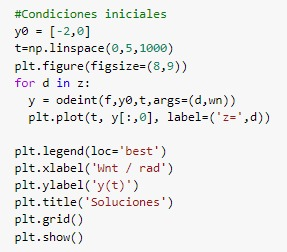
\includegraphics[height=12cm]{A2.jpeg}
 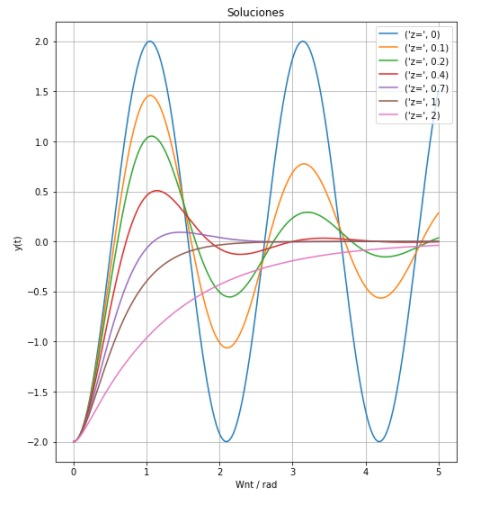
\includegraphics[height=15cm]{A3.jpeg} 
\end{center}



%-------------------------------------------------------------------


\section{Problema 2}

El en el caso #2, nos encontramos resolviendo numericamente el ejercicio, donde establecimos nuestros datos, sustituimos los valores, ingresamos algunas condiciones iniciales y llegamos a calcular las soluciones deseadas con su respectiva gráfica.\\


\begin{center}
 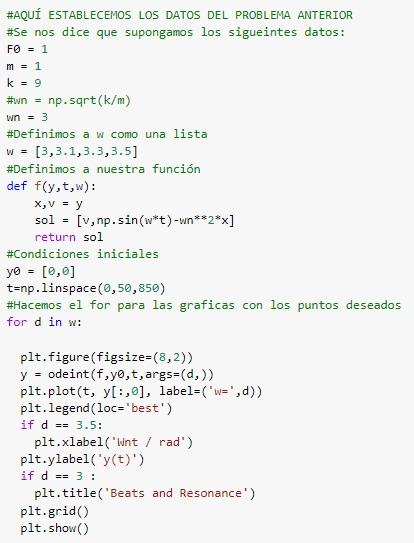
\includegraphics[height=20cm]{A4.jpeg}  
 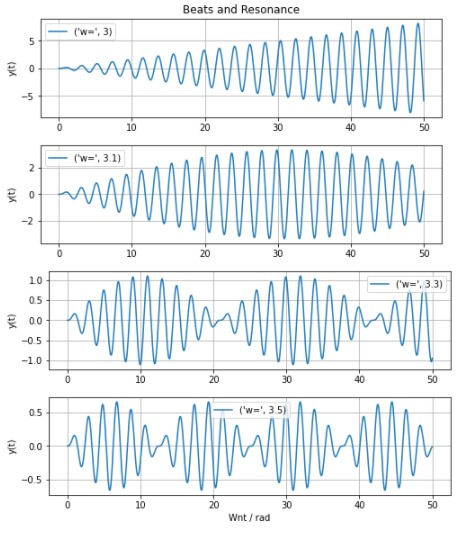
\includegraphics[height=18cm]{A5.jpeg}
\end{center}
 

%---------------------------------------------------------------



\section{Problema 3}

El en el caso #3, nos encontramos resolviendo numericamente el ejercicio, donde establecimos nuestros datos, sustituimos los valores, ingresamos algunas condiciones iniciales y llegamos a calcular las soluciones deseadas con su respectiva gráfica.\\

\begin{center}
    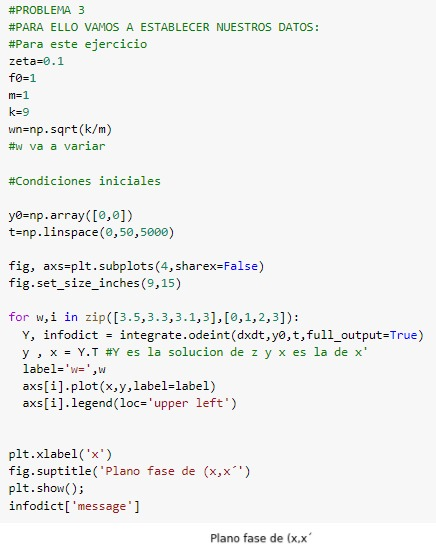
\includegraphics[height=20cm]{A6.jpeg}  
    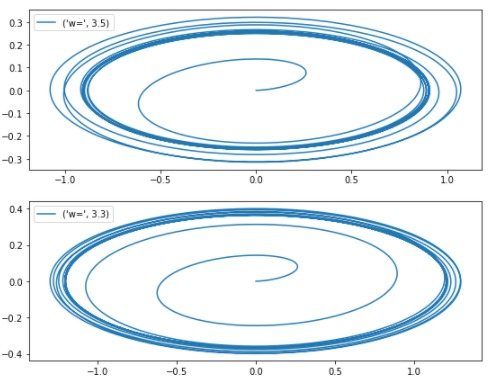
\includegraphics[height=13cm]{A7.jpeg}
	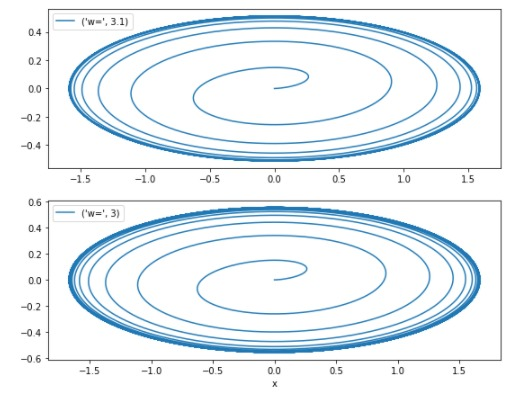
\includegraphics[height=12cm]{A8.jpeg}
\end{center}





%-------------------------------------------------------------------


\section*{Conclusión}


Al concluir esta actividad, podemos ver la gran funcionalidad que tienen estas bibliotecas para la hora de trabajar con estos datos, ya que con cada una de estas nos ayudó en una función específica. También podemos ver como es que las bibliotecas nos ayudaron en ciertas funciones especiales, como lo son el caso de los problemas 3, donde encontramos cosas o herramientas computacionales muy sofisticadas, es por eso que en esta actividad se repasaron los conocimientos adquiridos, y reforzamos todo el uso de ellos, es por eso que las actividades ayudaron en este tipo de situaciones. 


%---------------------------------------------------------------

\end{document}